Based on the techniques and functionalities described in 
the previous sections, we now show how to design and implement
a subdivision library for a generic CGAL polyhedron. This 
library is named as the \emph{C}ombinatorial \emph{S}ubdivision 
\emph{L}ibrary, short CSL. CSL contains a set of refinement 
functions and geomtry smoothing rules. Subdivisions 
are specilaized as a proper combination of the refinement 
schemes and the smoothing rules. The goals of CSL are the 
\emph{generic polyhedron data},
\emph{user-friendly functional forms}, 
\emph{user-customizable subdivsions}, and a
\emph{extendible library}. 

CSL is designed based on the policy-based design 
\cite{Alexandrescu:2001:MCD}.
The policy-based design assembles a class
(called \emph{host}) with complex behavior out of many 
small and generic behaviors (called \emph{policies}).
Each policy defines an interface for a
specific behavior and cumstomizable by the user. 
Policies are usually implemented as the functions or functors.
One gentle example is the \CodeFmt{for\_each} algorithm in STL 
\footnote{\path|http://www.sgi.com/tech/stl/for_each.html|}. 
\begin{lstlisting}
template <class InputIterator, class UnaryFunction>
UnaryFunction for_each(InputIterator first, InputIterator last, UnaryFunction f);
\end{lstlisting}
The \CodeFmt{UnaryFunction f} is the generic behavior cunstomizable 
by the user. 

Based on the policy-based design, CSL
is designed for both the generic types, i.e.\ the polyhedron,
and the generic behaviors, i.e.\ the subdivisions.
%This means users can customize the subdivisions at compile time. 
The interface of the generic types is specified as a \cgalpoly .
In addition to the connectivity interface like circulators or
the adjacency pointers of a halfedge, CSL requires the
\CodeFmt{Point\_3} of the vertex item. \CodeFmt{Point\_3} serves
as the only geometry interface of the polyhedron in CSL.

There are three key behaviors in a subdivision: \emph{refinement}, 
\emph{smoothing} and \emph{stencil correspondence}. The refinement is
acted as a \CodeFmt{for\_each} algorithm on the source \emph{and} refined
polyhedron while applying the smoothing behaviors. CSL implement the
refinements as the host functions with the smoothing rules as the
policies. Some major refinement schemes are shown in 
\figurename\ \ref{fig:RefSchemes}. The refinements also define the
stencil correspondences as shown in \figurename\ \ref{fig:RefMap}.
These stencil correspondences specified the policy interface 
between the refinements and the smoothing.

%% \cgalpoly\ provides two
%% mechanisms to implement refinements as introduced in the previous
%% sections. The geometry smoothing is mixed with the refinement
%% in the previous examples and hence implicitly maintain
%% the stencil correspondence. CSL extracts the geometry smoothing
%% from the refinement as policies and maintain the stencil 
%% correspondence explicitly. 



%-----------------------------------------------------------------------
\subsubsection{Primal Quad Quadralization}
Subdivisions in CSL is constructed as a
\emph{refinement function} parameterized with the 
\emph{geometry smoothing rules}. 

\begin{lstlisting}
void CatmullClark_subdivision(Polyhedron& p, int step = 1) {
  quad_quadralize_polyhedron(p, CatmullClark_rule<Polyhedron>(), step);
}

template <class _Poly>
class quadralize_rule {
public:
  void face_point_rule(Facet_handle, Point&) {};
  void edge_point_rule(Halfedge_handle, Point&) {};
  void vertex_point_rule(Vertex_handle, Point&) {};
};

template <class _Poly>
class CatmullClark_rule: quadralize_rule<_Poly> {...};
\end{lstlisting}

The refinement functions, i.e.\ the \CodeFmt{quad\_quadralize\_polyhedron} 
and the \CodeFmt{dualize\_polyhedron}, 
refine the control mesh, maintain the correspondence between the 
control mesh and refined mesh, and apply the smoothing stencils 
provided by the policy class, i.e.\ the \CodeFmt{CatmullClark\_rule} 
and the \CodeFmt{DooSabin\_rule}. 

\begin{lstlisting}
template <template <typename> class RULE>
void quad_quadralize_polyhedron(Polyhedron& p, RULE<Polyhedron> rule, int step) {
  for (int i = 0; i < step; i++) quad_quadralize_1step(p, rule);
}
\end{lstlisting}

\begin{figure}
  \centering
  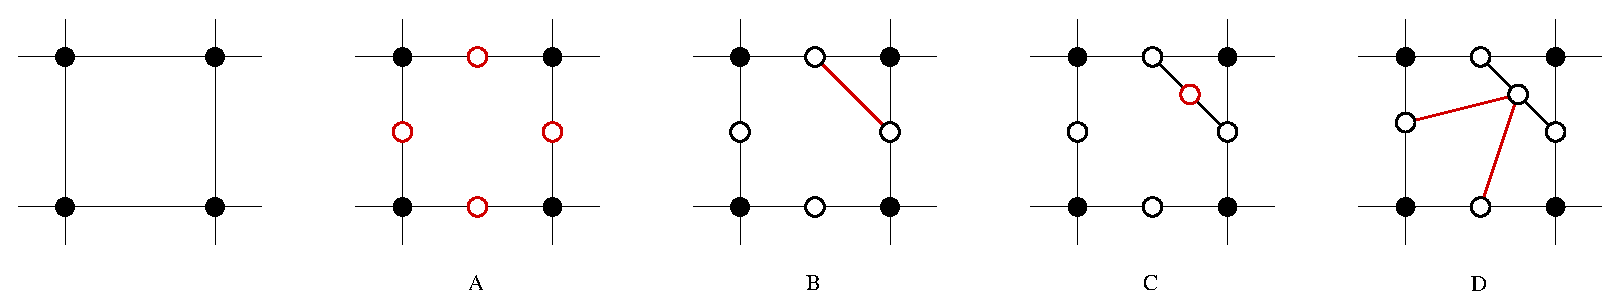
\epsfig{file=figs/CCRefinement.eps, width=10cm}
  \caption{A PQQ refinement of a facet is encoded into a sequence of
  vertex insertions and edge insertions. Red indicates the inserted
  vertices and edges in each step.}
  \label{fig:CCRefinement}
\end{figure}

\CodeFmt{quad\_quadralize\_polyhedron} is based on the Euler
operators. The operator sequence is pictured in 
\figurename\ \ref{fig:CCRefinement}.


The \CodeFmt{quadralize\_polyhedron<>()} 
is the host function refining the input mesh
and the \CodeFmt{CatmullClark\_rule} is the policy 
class applying the Catmull-Clark stencils.
The refinement functions are implemented based on the
Euler operations or the modifier callback mechanism.
The refinement functions also maintain the 
correspondence with the stencil, i.e., the submesh 
centered around the given facet, edge, or
vertex, and the smoothing point.
The smoothing point is calculated by calling the 
policies, e.g., the \CodeFmt{facet\_rule()}, the 
\CodeFmt{edge\_rule()}, and the \CodeFmt{vertex\_rule()} 
respectively. Inside a policy, applying the 
stencil is simplified to the mesh traversal of a 
1-ring neighborhood which can be done with the 
circulators. Following example illustrates  
the policy of the facet-stencil in Catmull-Clark 
subdivision.

\begin{lstlisting}
template <class _Poly>
class CatmullClark_rule : public quadralize_rule<_Poly> {
public:
  void face_point_rule(Facet_handle facet, Point& pt) {
    Halfedge_around_facet_circulator hcir = facet->facet_begin();
    int n = 0;
    Kernel::FT p[] = {0,0,0};
    do {
      Point t = hcir->vertex()->point();
      p[0] += t[0], p[1] += t[1], p[2] += t[2]; 
      ++n;
    } while (++hcir != facet->facet_begin());
    pt = Point(p[0]/n, p[1]/n, p[2]/n);
  }
  void edge_point_rule(Halfedge_handle edge, Point& pt) {
    Point p1 = edge->vertex()->point();
    Point p2 = edge->opposite()->vertex()->point();
    Point f1, f2;
    face_point_rule(edge->facet(), f1);
    face_point_rule(edge->opposite()->facet(), f2);
    pt = Point((p1[0]+p2[0]+f1[0]+f2[0])/4,
	       (p1[1]+p2[1]+f1[1]+f2[1])/4,
	       (p1[2]+p2[2]+f1[2]+f2[2])/4 );
  }
  void vertex_point_rule(Vertex_handle vertex, Point& pt) {
    Halfedge_around_vertex_circulator vcir = vertex->vertex_begin();
    int n = circulator_size(vcir);    

    float Q[] = {0.0, 0.0, 0.0}, R[] = {0.0, 0.0, 0.0};
    Point& S = vertex->point();
    
    Point q;
    for (int i = 0; i < n; i++, ++vcir) {
      Point& p2 = vcir->opposite()->vertex()->point();
      R[0] += (S[0]+p2[0])/2; R[1] += (S[1]+p2[1])/2; R[2] += (S[2]+p2[2])/2;
      face_point_rule(vcir->facet(), q);
      Q[0] += q[0]; Q[1] += q[1]; Q[2] += q[2];
    }
    R[0] /= n;    R[1] /= n;    R[2] /= n;
    Q[0] /= n;    Q[1] /= n;    Q[2] /= n;
      
    pt = Point((Q[0] + 2*R[0] + S[0]*(n-3))/n,
	       (Q[1] + 2*R[1] + S[1]*(n-3))/n,
	       (Q[2] + 2*R[2] + S[2]*(n-3))/n );
  }
\end{lstlisting}

\begin{lstlisting}
  void face_point_rule(Facet_handle facet, Point& pt) {
    Halfedge_around_facet_circulator hcir = facet->facet_begin();
    Vector vec = hcir->vertex()->point() - CGAL::ORIGIN;
    ++hcir;
    do {
      vec = vec + hcir->vertex()->point();
    } while (++hcir != facet->facet_begin());
    pt = CGAL::ORIGIN + vec/circulator_size(hcir);
  }
\end{lstlisting}

The circulator of the facet provides a convenient way to
traverse and collect the stencils. A more complicated
example is the edge-stencil in Catmull-Clark 
subdivision as following code,

A low lever halfedge traversal is used to locate the
adjacent facets of the edge and the circulators are used
to collect the repective facet vertives. The vertex-stencil
has the most complicated configuration since the
extra-ordinary vertex introduce dynamic weights. But the travesal
is still restruicted inside the 1-ring neighbors of the vertex
which can be collect easily with the vertex ciculator.

The refinement host employs the gemoetry policies
tp generate the smoothed point and applys them in the
proper vertives of the refined polyhedron. The key here is 
the correct stencil correspondence. Since CSL is designed
to accept a customized \cgalpoly , item flags in the 
Quad-Triangle example is not an option here.
To maintain the stencil correspondence, CSL implicitly
records the storage position. Note \cgalpoly\ allocates new
geometry items by appending them at the end of the underlying
containers, in most cases the linked-list or the vector.
Hence, the storage order can be encoded as the order of
the allocations and able to used to distincish the
stencil correspondence, e.g.\ facet to vertex, edge to facet
of vertex to vertex in Catmull-Clark subdivision.

\begin{lstlisting}
template <class _P> template <template <typename> class RULE>
void Polyhedron_subdivision<_P>::dualize_1step(_P& p, RULE<_P> rule) {
  int num_v = p.size_of_vertices();
  int num_e = p.size_of_halfedges()/2;
  int num_f = p.size_of_facets();
  int num_facet = num_v + num_e + num_f;
  
  // init the buffer for the next level
  Point* point_buffer = new Point[num_e*2];
  int** facet_buffer = new int*[num_facet];
  for (int i = 0; i < num_facet; ++i) facet_buffer[i] = NULL;

  // build the point_buffer
  Halfedge_iterator he_itr = p.halfedges_begin(); 
  for (int i = 0; i < num_e*2; ++i, ++he_itr) {
    Halfedge_around_facet_circulator cir = he_itr->facet_begin();
    rule.point_rule(cir, point_buffer[i]);
  }

  // build the facet_buffer
  he_itr = p.halfedges_begin(); 
  Facet_iterator fitr = p.facets_begin();  
  for (int i = 0; i < num_f; ++i, ++fitr) {
    Halfedge_around_facet_circulator  cir = fitr->facet_begin();
    int n =  CGAL::circulator_size(cir); 
    facet_buffer[i] = new int[n+1];
    facet_buffer[i][0] = n;
    for (int j = 1; j < n+1; ++j, ++cir)
      facet_buffer[i][j] = 
	std::distance(he_itr, Halfedge_handle(cir.operator->())); 
  }
  Halfedge_iterator eitr = p.halfedges_begin();
  for (int i = num_f; i < num_f+num_e; ++i, ++eitr) {
    facet_buffer[i] = new int[4+1];
    facet_buffer[i][0] = 4;
    facet_buffer[i][1] = (i-num_f)*2;
    facet_buffer[i][2] = std::distance(he_itr, eitr->prev());    
    ++eitr;
    facet_buffer[i][3] = (i-num_f)*2+1; 
    facet_buffer[i][4] = std::distance(he_itr, eitr->prev());    
  }
  Vertex_iterator vitr = p.vertices_begin();
  for (int i = num_f+num_e; i < num_f+num_e+num_v; ++i, ++vitr) {
    Halfedge_around_vertex_circulator  cir = vitr->vertex_begin();
    int n =  CGAL::circulator_size(cir); 
    facet_buffer[i] = new int[n+1];
    facet_buffer[i][0] = n;

    for (int j = 1; j < n+1; ++j, --cir)
      facet_buffer[i][j] = 
	std::distance(he_itr, Halfedge_handle(cir.operator->())); 
  }
  
  p.clear();
  Polyhedron_memory_builder<Polyhedron> pb(num_e*2, point_buffer, 
					   num_f+num_e+num_v, facet_buffer);
  p.delegate(pb);
  
  // release the buffer of the new level
  for (int i = 0; i < num_facet; ++i) delete[] facet_buffer[i];
  delete[] facet_buffer;
  delete[] point_buffer;
}
\end{lstlisting}


Following code demonstrates the stencil correspondence in
Catmull-Clark subdivision.



%-----------------------------------------------------------------------
\subsubsection{Dual Quad Quadralization}
\begin{lstlisting}
void DooSabin_subdivision(Polyhedron& p, int step = 1) {
  dualize_polyhedron(p, DooSabin_rule<Polyhedron>(), step);
}
template <class _Poly>
class dualize_rule {
public:
  void point_rule(Halfedge_around_facet_circulator cir, Point& pt) {};
};
\end{lstlisting}

\begin{lstlisting}
template <class _Poly>
class DooSabin_rule : public dualize_rule<_Poly> {
public:
  void point_rule(Halfedge_around_facet_circulator cir, Point& pt) {
    int n =  CGAL::circulator_size(cir); 

    Vector cv(0,0,0), t;
    if (n == 4) {
      cv = cv + (cir->vertex()->point()-CGAL::ORIGIN)*9;
      cv = cv + ((++cir)->vertex()->point()-CGAL::ORIGIN)*3;
      cv = cv + ((++cir)->vertex()->point()-CGAL::ORIGIN);
      cv = cv + ((++cir)->vertex()->point()-CGAL::ORIGIN)*3;
      cv = cv/16;
    } else {
      double a;
      for (int k = 0; k < n; ++k, ++cir) {
	if (k == 0) a = ((double)5/n) + 1;
	else a = (3+2*std::cos(2*k*3.141593/n))/n;
	cv = cv + (cir->vertex()->point()-CGAL::ORIGIN)*a;
      }
      cv = cv/4;
    }
    pt = CGAL::ORIGIN + cv;
  }
};
\end{lstlisting}

Some refinement schemes is not easy to devise a sequence
of the Euler operations. For example the Doo-Sabin subdivision.
Fot these schemes, the refinements are supported based on the
modifier callback mechanism (MCM). In the example of 
Quad-Triangle subdivision, MCM is used to devise 
customized Euler-like atomic operators.
In CSL, MCM is used to \emph{rebuild} the refinement
mesh based on simplified mesh data, e.g.\ facet-vertex index list.
The facet-vertex index list is build based on the encoded order
of the connectivity. It is demonstrated in the following code,

\begin{lstlisting}
template <template <typename> class RULE>
void dualize_polyhedron(Polyhedron& p, RULE<Polyhedron> rule, int step = 1) {
  for (int i = 0; i < step; ++i) dualize_1step(p, rule);
}
\end{lstlisting}


\begin{lstlisting}
template <class _P> template <template <typename> class RULE>
void Polyhedron_subdivision<_P>::dualize_1step(_P& p, RULE<_P> rule) {
  int num_v = p.size_of_vertices();
  int num_e = p.size_of_halfedges()/2;
  int num_f = p.size_of_facets();
  int num_facet = num_v + num_e + num_f;
  
  // init the buffer for the next level
  Point* point_buffer = new Point[num_e*2];
  int** facet_buffer = new int*[num_facet];
  for (int i = 0; i < num_facet; ++i) facet_buffer[i] = NULL;

  // build the point_buffer
  Halfedge_iterator he_itr = p.halfedges_begin(); 
  for (int i = 0; i < num_e*2; ++i, ++he_itr) {
    Halfedge_around_facet_circulator cir = he_itr->facet_begin();
    rule.point_rule(cir, point_buffer[i]);
  }

  // build the facet_buffer
  he_itr = p.halfedges_begin(); 
  Facet_iterator fitr = p.facets_begin();  
  for (int i = 0; i < num_f; ++i, ++fitr) {
    Halfedge_around_facet_circulator  cir = fitr->facet_begin();
    int n =  CGAL::circulator_size(cir); 
    facet_buffer[i] = new int[n+1];
    facet_buffer[i][0] = n;
    for (int j = 1; j < n+1; ++j, ++cir)
      facet_buffer[i][j] = 
	std::distance(he_itr, Halfedge_handle(cir.operator->())); 
  }
  Halfedge_iterator eitr = p.halfedges_begin();
  for (int i = num_f; i < num_f+num_e; ++i, ++eitr) {
    facet_buffer[i] = new int[4+1];
    facet_buffer[i][0] = 4;
    facet_buffer[i][1] = (i-num_f)*2;
    facet_buffer[i][2] = std::distance(he_itr, eitr->prev());    
    ++eitr;
    facet_buffer[i][3] = (i-num_f)*2+1; 
    facet_buffer[i][4] = std::distance(he_itr, eitr->prev());    
  }
  Vertex_iterator vitr = p.vertices_begin();
  for (int i = num_f+num_e; i < num_f+num_e+num_v; ++i, ++vitr) {
    Halfedge_around_vertex_circulator  cir = vitr->vertex_begin();
    int n =  CGAL::circulator_size(cir); 
    facet_buffer[i] = new int[n+1];
    facet_buffer[i][0] = n;

    for (int j = 1; j < n+1; ++j, --cir)
      facet_buffer[i][j] = 
	std::distance(he_itr, Halfedge_handle(cir.operator->())); 
  }
  
  p.clear();
  Polyhedron_memory_builder<Polyhedron> pb(num_e*2, point_buffer, 
					   num_f+num_e+num_v, facet_buffer);
  p.delegate(pb);
  
  // release the buffer of the new level
  for (int i = 0; i < num_facet; ++i) delete[] facet_buffer[i];
  delete[] facet_buffer;
  delete[] point_buffer;
}
\end{lstlisting}


%-----------------------------------------------------------------------
\subsubsection{CSL}
This policy-based approach offers a convenient way to
specialize a subdivision with the template smoothing rules.
CSL currently supports Catmull-Clark, 
Loop, Doo-Sabin, $\sqrt{3}$ and Quad-Triangle
subdivisions. %(\figurename\ \ref{fig:subzoo}).
Though demonstrated with a specific enriched \poly\ in our 
polyhedron viewer, CSL accepts any polyhedron mesh specialized 
from the \poly\ with the \CodeFmt{Point} type defined in the vertex.  
Subdivisions in CSL are build as proper combinations of the
refinement functions and the geometry policy classes.
The proper combination is constrained by the stencil correspondence.

Current version of CSL only supports the geometry modification 
of the vertex (hence only the isotrophic subdivision). Boundary
can be easily supported by introducing the boundary policy. But
for anisotrophic subdivisions (e.g.\ Pixar's crease rules), data
modifications of the halfedge are required. It can be done by 
introduce halfedge policy, though a much complex structures
is need in the refinement host.


\begin{lstlisting}
  template <template <typename> class RULE>
  static void quad_quadralize_1step(Polyhedron& p, RULE<Polyhedron> rule);
  template <template <typename> class RULE>
  static void tri_quadralize_1step(Polyhedron& p, RULE<Polyhedron> rule);
  template <template <typename> class RULE>
  static void dualize_1step(Polyhedron& p, RULE<Polyhedron> rule);
\end{lstlisting}


